\documentclass{beamer}
\usetheme{Warsaw}

\usepackage[utf8]{inputenc}
\usepackage{fancybox}
\usepackage{multimedia} 
\usepackage{subfig}
\usepackage{amsmath}
\usepackage{hyperref}
\usepackage[all]{xy}
\begin{document}


\title[Stochastik] % (optional, only for long titles)
{Stochastik für Informatiker
\\
\includegraphics[scale=0.5]{img/craps}
}
\subtitle{}
\author[Dr. Johannes Riesterer] % (optional, for multiple authors)
{Dr.  rer. nat. Johannes Riesterer}

\date[KPT 2004] % (optional)
{}

\subject{Stochastik}


\frame{\titlepage}

\begin{frame}
    \frametitle{Verteilungen}
\framesubtitle{}

\begin{block}{Verteilung}
Sei $(\mathbb{R}, \mathcal{B}, P)$ ein Wahrscheinlichkeitsraum über $\mathbb{R}$ mit Borell'scher $\sigma$-Agebra $\mathcal{B}$. Die Abbildung
\begin{align*}
F_P (x)  = P((-\infty, x ])
\end{align*}
wird Wahrscheinlichkeitsverteilung genannt.
\end{block}

\begin{block}{Verteilung einer Zufallsvariablen}
Ist $(\Omega, \mathcal{A}, P)$ ein Wahrscheinlichkeitsraum und $X : \Omega \to \mathbb{R}$ eine reelle Zufallsvariable, so erhalten wir die zugehörige Wahrscheinlichkeitsverteilung
\begin{align*}
F_X (x)  = P_X(  X \leq x)  \; .
\end{align*}
Ist $f$ eine Dichte auf $\mathbb{R}$ und $F_X = P_f$ so schreiben wir  auch $X \sim P_f$
\end{block}
 \end{frame}


\begin{frame}
    \frametitle{Verteilungen}
\framesubtitle{}

\begin{block}{Verteilung}
Ist $f: \mathbb{R} \to [0,1]$ eine dichte und $P_f$ das zugehörige Wahrscheinlichkeitsmaß, dann gilt 
\begin{align*}
\frac{d}{dx} F_{P_f} (x)  = f(x)
\end{align*}
(Hauptsatz der Integral- und Differentialrechnung)
\end{block}
 \end{frame}



\begin{frame}
    \frametitle{Verteilungen}
\framesubtitle{}

\begin{block}{Gleichverteilung}
Die Gleichverteilung $U{(a,b)}$ auf einem Intervall $(a,b) \subset \mathbb{R}$ ist definiert durch
\begin{align*}
& \text{Dichte: } f (x) : = \frac{1_{(a,b)}}{|a-b| } \\
& \Rightarrow \text{Verteilung: } F (x) =  P_f( (-\infty, x))  =  \int_{-\infty}^{x} \frac{1_{(a,b)}}{|b-a|} dt\\\
& = \begin {cases} 0 \text{ für } x \leq a \\   \frac{x-a}{|b-a|} \text{ für } a \leq x \leq b \\ 1 \text{ für }  x \geq b \\  \end{cases}
\end{align*}
\end{block}

 \end{frame}

\begin{frame}
    \frametitle{Verteilungen}
\framesubtitle{}

\begin{figure}[htp]
      \centering
    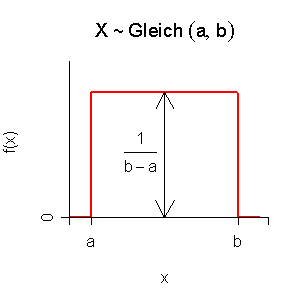
\includegraphics[width=0.42\textwidth]{img/gleichverteilung1}
    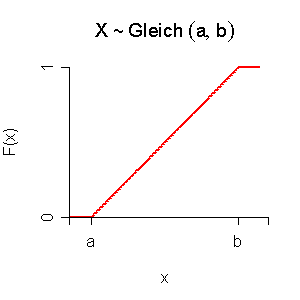
\includegraphics[width=0.42\textwidth]{img/gleichverteilung2}
      \caption{Quelle: Wikipedia}
\end{figure}
 \end{frame}




\begin{frame}
    \frametitle{Verteilungen}
\framesubtitle{}

\begin{block}{Gleichverteilung}
Sei $X \sim $U(a,b).
\begin{align*}
& \mathbb{E}(X) =\int\limits_{-\infty}^\infty xf(x)\,dx = \frac 1{b-a}\int\limits_a^b x\cdot 1\,dx = \frac 12\frac{b^2-a^2}{b-a} = \frac{a+b}2 \\
& \mathbb{V}(X) = \operatorname{E}(X^2) - \left({\operatorname{E}(X)} \right)^2  = \frac{1}{b - a}\int\limits_a^b {x^2 \cdot 1\,dx}  - \left( {\frac{a + b}{2}} \right)^2  \\
 & = \frac{1}{3}\frac{b^3  - a^3}{b - a} - \left( {\frac{a + b}{2}} \right)^2 \\
    &= \frac{1}{12}\left( {4b^2  + 4ab + 4a^2  - 3a^2  - 6ab - 3b^2 } \right) = \frac{1}{12}(b - a)^2
\end{align*}
\end{block}
 \end{frame}



\begin{frame}
    \frametitle{Verteilungen}
\framesubtitle{}

\begin{block}{Normalverteilung}
Die Normalverteilung $N{(\mu,\sigma^2)}$ auf $\mathbb{R}$ ist definiert durch
\begin{align*}
& \text{Dichte: } f (x) : = \frac 1{\sigma \sqrt{2\pi}}e^{- \frac {1}{2} (\frac{x- \mu}{ \sigma})^2} \\
&  \Rightarrow \text{Verteilung: } F(x) = N{(\mu,\sigma^2)}(-\infty , x) =  \int_{-\infty}^{x}  \frac 1{\sigma \sqrt{2\pi}}e^{- \frac {1}{2} (\frac{t- \mu}{ \sigma})^2}dt\\
\end{align*}

\end{block}
 \end{frame}



\begin{frame}
    \frametitle{ Verteilungen}
\framesubtitle{}
\begin{figure}[htp]
      \centering
    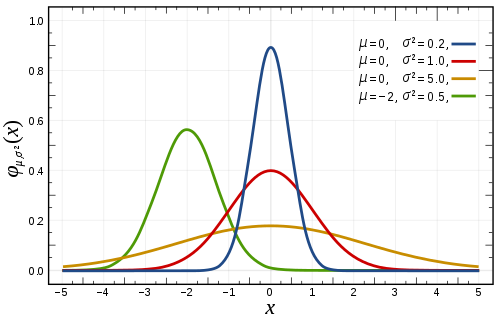
\includegraphics[width=0.45\textwidth]{img/normal}
    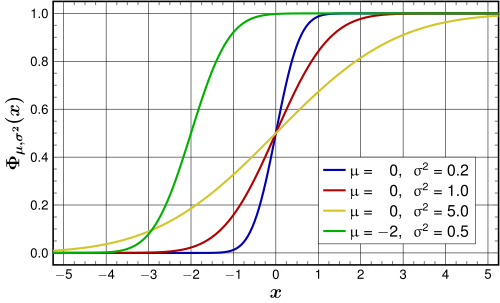
\includegraphics[width=0.45\textwidth]{img/normaldist}
      \caption{Quelle: Wikipedia}
\end{figure}

 \end{frame}


\begin{frame}
    \frametitle{Verteilungen}
\framesubtitle{}

\begin{block}{Normalverteilung}
Sei $X \sim N(\mu, \sigma)$.
\begin{align*}
& \mathbb{E}(X) = \mu \\
& \mathbb{V}(X) = \sigma^2
\end{align*}
\end{block}
 \end{frame}



\begin{frame}
    \frametitle{ Verteilungen}
\framesubtitle{}

\begin{block}{Poissonverteilung}
Die Poissonverteilung  $Pois (\lambda)$ auf $\mathbb{N}_{\geq 0}$ ist definiert durch
\begin{align*}
& P_\lambda (k) = \frac{\lambda^k}{k!}\, \mathrm{e}^{-\lambda} \\
& \Rightarrow F_{\lambda}(n)=\sum_{k=0}^n P_\lambda (k) = \mathrm{e}^{-\lambda} \sum_{k=0}^n \frac{\lambda^k}{k!}
\end{align*}
\end{block}
\begin{figure}[htp]
      \centering
    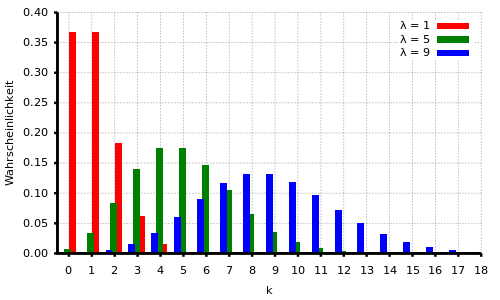
\includegraphics[width=0.55\textwidth]{img/Poisson}
      \caption{Quelle: Wikipedia}
\end{figure}
 \end{frame}



\begin{frame}
    \frametitle{ Verteilungen}
\framesubtitle{}

\begin{block}{Poisson Verteilung}
Die Poisson Verteilung beschreibt das Auftreten von seltenen Ereignissen und spielt bei Zählprozessen eine wichtige Rolle.
\end{block}
\begin{block}{Poisson Verteilung}
$X\sim Pois (\lambda)$ 
\begin{align*}
& \mathbb{E}(X) = \lambda \\
& \mathbb{V}(X) = \lambda
\end{align*}
\end{block}
 \end{frame}


\begin{frame}
    \frametitle{Verteilungen}
\framesubtitle{}

\begin{block}{Bernoulliverteilung}
Die Bernoulliverteilung  Für $\Omega = \{ 0, 1\}$ und $p \in [0,1]$ ist definiert durch
\begin{align*}
P (\omega) = p^{\omega} (1-p)^{1 -\omega}
\end{align*}
\end{block}

\begin{block}

\begin{itemize}
\item Werfen einer Münze: Kopf (Erfolg), $p=1/2$, und Zahl (Misserfolg), $q=1/2$.
\item Werfen eines Würfels, wobei nur eine 6 als Erfolg gewertet wird: $p=1/6, q=5/6$.
\item Qualitätsprüfung (einwandfrei, nicht einwandfrei).
\item Betrachte sehr kleines Raum/Zeit-Intervall: Ereignis tritt ein $(p \gtrapprox 0)$, tritt nicht ein $(q\lessapprox 1)$.
\end{itemize}

\end{block}
 \end{frame}




\begin{frame}
    \frametitle{ Verteilungen}
\framesubtitle{}

\begin{block}{Binomialverteilung}
\end{block}

\begin{figure}[htp]
      \centering
    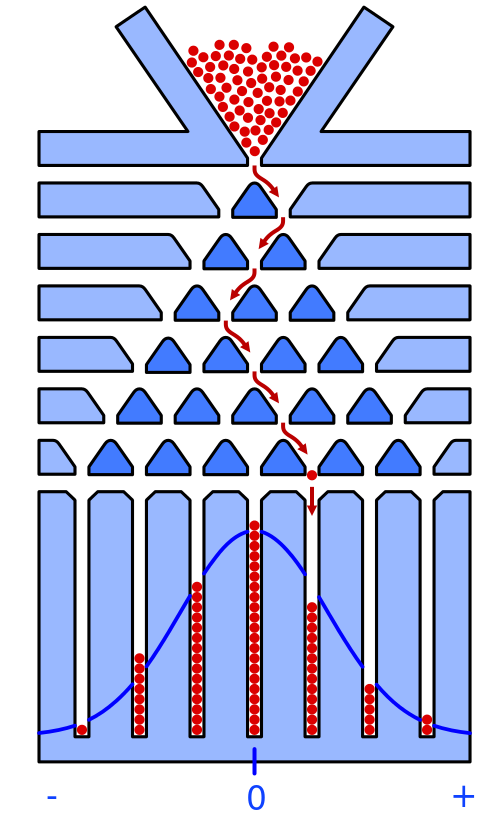
\includegraphics[width=0.25\textwidth]{img/Galton}
      \caption{Quelle: Wikipedia}
\end{figure}
 \end{frame}




\begin{frame}
    \frametitle{Statistik - Parameterschätzung}
\framesubtitle{}

\begin{block}{Erraten des Bereichs von Zufallsvariablen}
Angenommen man findet einen Apparat (Fluxkompensator?), der zufällig Zahlen in einem Intervall $[0, \rho]$ ausgibt. Anhand von Beobachtungen der Zahlen möchte man $\rho$ schätzen.
\end{block}

\begin{figure}[htp]
      \centering
    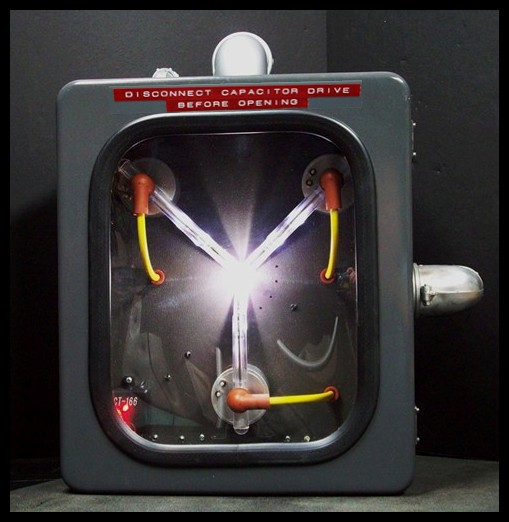
\includegraphics[width=0.35\textwidth]{img/flux}
      \caption{Quelle: forevergeek}
\end{figure}
 \end{frame}


\begin{frame}
    \frametitle{Statistik - Parameterschätzung}
\framesubtitle{}

\begin{block}{Erraten des Bereichs von Zufallsvariablen - Modell}
 Wir machen die Annahme, dass alle Zahlen in dem Intervall gleich wahrscheinlich auftreten und  nehmen $n$ Stichproben $X_1, \cdots, X_n$.
Einen Schätzer für $\rho$ bezeichnen wir mit $T_n$.
\end{block}

\begin{block}{Erraten des Bereichs von Zufallsvariablen - Schätzer 1}
Eine einfache und einleuchtende Idee ist es, $\rho$ durch die größte beobachtete Zahl zu schätzen, also
$T_n^{max} := \max(X_1, \cdots, X_n)$.
 \end{block}

\begin{block}{Erraten des Bereichs von Zufallsvariablen - Schätzer 2}
Da das Auftreten der Zahlen gleich wahrscheinlich ist, ist der Erwartungswert des Zufallsexperiments $\rho /2$. Unter Berufung auf das  schwache Gesetz der Großen Zahlen erscheint der Schätzer
$T_n^{E} :=  2 \cdot \biggl( \frac{1}{n} \sum_{i=1}^n X_i \biggr)$ sehr plausibel.
 \end{block}

 \end{frame}




\begin{frame}
    \frametitle{Statistik - Parameterschätzung}
\framesubtitle{}

\begin{block}{Erraten des Bereichs von Zufallsvariablen - Vergleich}
Welcher Schätzer ist besser und in welchem Sinn?
\end{block}

\begin{block}{Erraten des Bereichs von Zufallsvariablen - Vergleich Konvergenz}
\begin{align*}
& P(| T_n^{max} - \rho | \geq \epsilon)   = P(T_n^{max} \leq \rho - \epsilon)   \\
& = P(X_1  \leq \rho - \epsilon, \cdots,  X_n \leq \rho - \epsilon )  = (\frac{\rho - \epsilon}{\rho})^n \underset{n \to \infty}{\longrightarrow} 0
\end{align*}
\end{block}


\begin{block}{Erraten des Bereichs von Zufallsvariablen - Vergleich Konvergenz}
\begin{align*}
& P(| T_n^{E} - \rho | \geq \epsilon)   = P(| \frac{1}{n} \sum X_i  - \frac{\rho}{2} | \geq \frac{\epsilon}{2})  \underset{n \to \infty}{\longrightarrow} 0 \\
 & \text{(Gesetz der Großen Zahlen)}
\end{align*}
\end{block}

 \end{frame}


\begin{frame}
    \frametitle{Statistik - Parameterschätzung}
\framesubtitle{}


\begin{block}{Erraten des Bereichs von Zufallsvariablen - Vergleich Erwartungswert}
Da $P( T_n^{max}  \leq c) = (\frac{c}{\rho})^n $ und  $\frac{d}{dx} (\frac{c}{\rho})^n = \frac{n}{\rho^n} x^{n-1} $ und damit
\begin{align*}
& \mathbb{E}(T_n^{max} ) = \int_{0}^{\rho} x \frac{n}{\rho^n} x^{n- 1} \; dx  = \frac{n}{\rho^n} \int_{0}^{\rho} x^n \; dx = \frac{n}{n+1} \rho    \underset{n \to \infty}{\longrightarrow} \rho
\end{align*}
\end{block}

\begin{block}{Erraten des Bereichs von Zufallsvariablen - Vergleich Erwartungswert}
\begin{align*}
& \mathbb{E}(T_n^{E} ) = \frac{2}{n} \sum \mathbb{E}(X_i)   = \rho
\end{align*}
\end{block}
 \end{frame}




\begin{frame}
    \frametitle{Statistik - Parameterschätzung}
\framesubtitle{}

\begin{block}{Erraten des Bereichs von Zufallsvariablen - Vergleich Varianz}
\begin{align*}
& \mathbb{V}(T_n^{max} ) = \frac{4}{n} \mathbb{V}(X_1)   =  \frac{4}{n \rho}   \int_{0}^{\rho } (x - \frac{\rho}{2})^2 \; dx = \frac{\rho^2}{3n}
\end{align*}
\end{block}
\begin{block}{Erraten des Bereichs von Zufallsvariablen - Vergleich Varianz}
\begin{align*}
& \mathbb{V}(T_n^{E} ) = \mathbb{E}((T_n^{E})^2 ) - (\mathbb{E}(T_n^{E} ))^2   \\
& = \int_{0}^{\rho} x^2 \frac{n}{\rho^n} x^{n- 1} \; dx - (\frac{n \rho}{n+1})^2 = \frac{n \rho^2}{(n+1)^2 (n+2)} 
\end{align*}
\end{block}
 \end{frame}







\begin{frame}
    \frametitle{Statistik - Parameterschätzung}
\framesubtitle{}

\begin{block}{Statistisches Modell}
Ein statistisches Modell ist ein Tripel $(\mathcal{X}, \mathcal{F}, P_\rho :  \rho \in \Theta)$ bestehend aus einer $\sigma$-Algebra $\mathcal{F}$ über dem Grundraum $\mathcal{X}$ und einer indizierten Menge (mit mindestens zwei Elementen) von Maßen $\{ P_\rho\}_{\rho \in \Theta}$. Für $\Theta \subset \mathbb{R}^n$ bezeichnet man es auch als parametrisiertes statistisches Modell. 
\end{block}

\begin{block}{Statistik}
Sei   $(\mathcal{X}, \mathcal{F}, P_\rho :  \rho \in\Theta)$ ein statistisches Modell und $(\Sigma, \mathcal{G})$ eine $\sigma$-Algebra über $\Sigma$. Eine Zufallsvariable 
\begin{align*}
X : \mathcal{X} \to \Sigma
\end{align*}
wird Statistik für  $(\mathcal{X}, \mathcal{F}, P_\rho :  \rho \in \Theta)$  genannt.
\end{block}
 \end{frame}



\begin{frame}
    \frametitle{Statistik - Parameterschätzung}
\framesubtitle{}

\begin{block}{Schätzer}
Sei   $(\mathcal{X}, \mathcal{F}, P_\rho :  \rho \in \Theta)$ ein statistisches Modell, $(\Sigma, \mathcal{G})$ eine $\sigma$-Algebra über $\Sigma$ und  
\begin{align*}
& \tau : \Theta \to \Sigma \\
 & \rho \mapsto \tau(\rho) 
\end{align*}
eine Abbildung. Eine Statistik   $T: \mathcal{X} \to \Sigma$  wird Schätzer für $\tau$ genannt.
\end{block}
 \end{frame}


\begin{frame}
    \frametitle{Statistik - Parameterschätzung}
\framesubtitle{}

\begin{block}{Konsistenz}
Eine Schätzfolge $T_n: \mathcal{X} \to \Sigma$  heißt konsistent, falls
\begin{align*}
P( |T_n - \tau(\rho)  |  \geq \epsilon)  \underset {n \to \infty}{\longrightarrow} 0 \text{ für alle } \epsilon > 0 \text { und alle } \tau \in \theta  
\end{align*}
also $T_n \to \tau(\rho)$ für $n \to \infty$  (stochastisch).
\end{block}
\begin{block}{Konsistenz}
Ein Schätzer $T: \mathcal{X} \to \Sigma$  heißt Erwartungstreu (unbiased), falls
\begin{align*}
\mathbb{E}(T) = \tau(\rho) \text{ für alle } \rho \in \theta.
\end{align*}
Andernfalls heißt $\mathbb{E}(T) - \tau(\rho) $ der Bias oder der systematische Fehler.
\end{block}
 \end{frame}

\begin{frame}
    \frametitle{Statistik - Parameterschätzung}
\framesubtitle{}
\begin{block}{Stichprobenmittel und  Stichprobenvarianz}
Für $n \geq 2$ sei  $\biggl ( \mathbb{R}^n, \mathcal{B}(\mathbb{R}^n ), P^n_\rho :=  \prod (P_\rho)_i \biggr)$ das Produktmodell,  $X: \mathbb{R \to \mathbb{R}}$ eine Zufallsvariable, $X_i(x_1, \cdot ,x_n) = x_i$ die Projektion auf die $i$-te Koordinate  und $m(\rho) = \mathbb{E}(X) $ so wie $v(\rho) =\mathbb{V}(X)$. Des weiteren seien  $X$ so wie $X_i$  unabhängig und identisch verteilt. Dann sind das Stichprobenmittel $M= \frac{1}{n} \sum_{i=1}^n X_i$ und die Stichprobenvarianz
 $V= \frac{1}{n-1} \sum_{i=1}^n (X_i - M)^2$ erwartungstreue Schätzer für $m$ bzw. $v$.
\end{block}

\begin{block}{Beweis}
Sei $\rho \in \Theta$ fest. Wegen linearität des EW und u.i.v. ist $\mathbb{E}(V) =\frac{1}{n} \sum_{i=1}^n \mathbb{E}(X_i) = m(\rho) $.
\end{block}


 \end{frame}


\begin{frame}
    \frametitle{Statistik - Parameterschätzung}
\framesubtitle{}

\begin{block}{Beweis}
Aus Linearität des EW und $\mathbb{E}(X_i - M) = 0$, u.i.v, stochastische Unabhängigkeit folgt
\begin{align*}
&(n-1) \mathbb{E}(V)  = \sum_{i=1}^n  \mathbb{V}(X_i - M) \\
& = n   \mathbb{V} (\frac{n-1}{n} X_1  - \frac{1}{n} \sum_{j=2}^n X_j) \\
& = n((\frac{n-1}{n})^2 + (n-1) \frac{1}{n^2}  ) v(\rho) = (n-1) v(\rho)
\end{align*}
Durch Teilen beider Seiten durch $n-1$ folgt die Behauptung. 
\end{block}


 \end{frame}




\begin{frame}
    \frametitle{Statistik - Parameterschätzung}
\framesubtitle{}

\begin{block}{Likelyhood Funktion}
Für eine parametrisierte Dichte $p_\rho : \mathcal{X}   \to  [0,1]$ heißt die Funktion
\begin{align*}
& p  : \mathcal{X}  \times  \Theta  \to  [0,1] \\
& p(x, \rho) := p_\rho (x)
\end{align*}
die zugehörige Likelyhood Funktion und 
\begin{align*}
& p_x  : \Theta   \to  [0,1] \\
& p_x(\rho):=  p(x, \rho) 
\end{align*}
die Liekelyhood Funktion zum Beobachtungswert $x \in \mathcal{X}$.

Im diskreten Fall setzten wir $ p(x, \rho) := P_\rho (\{ x\})$
\end{block}
 \end{frame}



\begin{frame}
    \frametitle{Statistik - Parameterschätzung}
\framesubtitle{}
\begin{block}{Maximum Likelyhood Schätzer}
Ein Schätzer $T: \mathcal{X} \to \Sigma$ heißt Maximum-Likelyhood-Schätzer, falls
\begin{align*}
p(x , T(x)) = \max_{\rho \in \Theta} p (x, \rho) \text{ für alle } x \in \mathcal{X}
\end{align*}
also der Schätzwert $T(x)$ eine Maximalstelle der Funktion  $p_x$ auf $\Theta$ ist.
\end{block}

 \end{frame}



\begin{frame}
    \frametitle{Statistik - Parameterschätzung}
\framesubtitle{}
\begin{block}{Erraten des Bereichs von Zufallsvariablen - Maximum Likelyhood-Schätzer}
Die Likelyhood Funktion ist hier gegeben durch
\begin{align*}
p_x (\rho) =  \begin{cases}  \frac{1}{\rho^n}  \text{ falls }  x_1, \cdots , x_n \leq \rho  \\  0  \text{ sonst}\end {cases}
\end{align*}
Somit ist der Schätzer $T_n^{max} (x) := \max (x_1, \cdots , x_n )$ der Maximum-Likelyhood-Schätzer.
\end{block}

 \end{frame}




\begin{frame}
    \frametitle{Statistik - Parameterschätzung}
\framesubtitle{}
\begin{block}{Physikalische Messung - Maximum Likelyhood-Schätzer}
Gegeben ist ein Sensor mit einer unbekannten Messgenauigkeit. Wir nehmen deshalb an, dass die Messung des Sensors einer Normalverteilung folgt, 
wobei der Erwartungswert (Messwert) und die Varianz (Streuung um Messwert) unbekannt sind. Wir machen $n$ unabhängige Messungen und erhalten damit das Normalverteilte Produktmodell $\bigl(\mathbb{R}^n, \mathcal{B}(\mathbb{R}^n), \prod_{i=1}^n N(m,v): m \in \mathbb{R}, v  >0 \bigr)$. 

\end{block}

 \end{frame}



\begin{frame}
    \frametitle{Statistik - Parameterschätzung}
\framesubtitle{}
\begin{block}{Physikalische Messung - Maximum Likelyhood-Schätzer}
Die Likelyhood-Funktion ist gegeben durch
\begin{align*}
p_x(\rho) =  \prod_{i=1}^n \frac {1}{ \sqrt{2 \pi v }} e^{- \frac{(x_i- m)^2}{ 2v}} =  \frac {1}{ \sqrt{2 \pi v }} e^{- \sum_{i=1}^n \bigl( \frac{(x_i- m)^2}{ 2v} \bigr)} 
\end{align*} 
mit $x = (x_1, \cdots, x_n)$ und $\rho=(m,v)$.
\end{block}

\begin{block}{Physikalische Messung - Maximum Likelyhood-Schätzer}
Um diesen Ausdruck zu maximieren, muss $m$ so gewählt werden, dass die quadratische Fehlersumme $ \sum_{i=1}^n (x_i- m)^2$ minimal wird.  Das ist der Fall für $m= M(x)= \frac{1}{n} \sum_{i=1}^n x_i$.
\end{block}

 \end{frame}

\begin{frame}
    \frametitle{Statistik - Parameterschätzung}
\framesubtitle{}
\begin{block}{Physikalische Messung - Maximum Likelyhood-Schätzer}
Des weiteren muss $v$ so gewählt werden, dass $ \frac {1}{ \sqrt{2 \pi v }} e^{- \sum_{i=1}^n \bigl( \frac{(x_i- M(x))^2}{ 2v} \bigr)}$ maximal wird. Differenziert man den Logarithmus dieses Ausdrucks nach $v$, erhalten wir
\begin{align*}
& -\frac{d}{dv} (\frac{n}{2} \log(v) + \frac{1}{2v} \sum_{i=1}^n (x_i - M(x))^2 ) \\
& = -\frac{n}{2v} + \frac{1}{2v^2}\sum_{i=1}^n (x_i - M(x))^2 
\end{align*}
Dieser Term ist maximal, falls der letzte Term verschwindet. Dies ist er Fall für
$v = V(x) =\frac{1}{n}\sum_{i=1}^n (x_i - M(x))^2$
\end{block}

 \end{frame}








\end{document}
